%
% test_report_v05.tex
%
% Copyright (C) 2021 by SpaceLab.
%
% EPS 2.0 Documentation
%
% This work is licensed under the Creative Commons Attribution-ShareAlike 4.0
% International License. To view a copy of this license,
% visit http://creativecommons.org/licenses/by-sa/4.0/.
%

%
% \brief Test report of the v0.1 hardware.
%
% \author André M. P. Mattos <andre.mattos@spacelab.ufsc.com>
%
% \institution Universidade Federal de Santa Catarina (UFSC)
%
% \version 0.1.0
%
% \date 2021/06/23
%

\chapter{Test Report of v0.1 Version} \label{anx:test-report-v01}

This appendix is a test report of the first manufactured and assembled PCB (version v0.1).

\begin{itemize}
    \item \textbf{PCB manufacturer}: PCBWay (China)
    \item \textbf{PCB assembly}: PCBWay (China)
    \item \textbf{PCB arrival date}: 2021/04/14
    \item \textbf{Execution date}: 2021/06/13 to 2021/07/01
    \item \textbf{Tester}: André M. P. Mattos
\end{itemize}



\section{Visual Inspection}

\begin{figure}[!ht]
    \begin{center}
        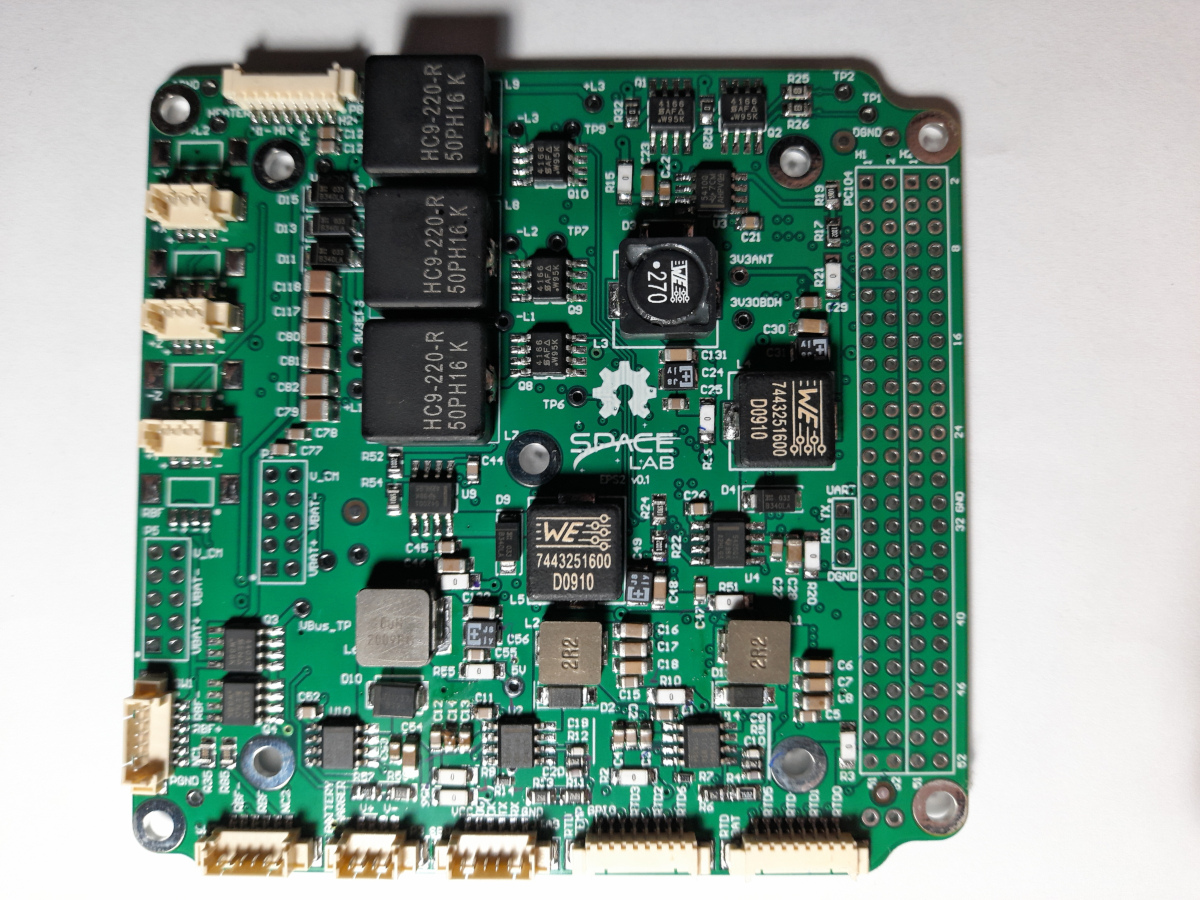
\includegraphics[width=0.75\columnwidth]{figures/v01/eps2-v01-top.jpg}
        \caption{Top view of the EPS 2.0 v0.1 board.}
        \label{fig:eps2-v01-top}
    \end{center}
\end{figure}

\begin{figure}[!ht]
    \begin{center}
        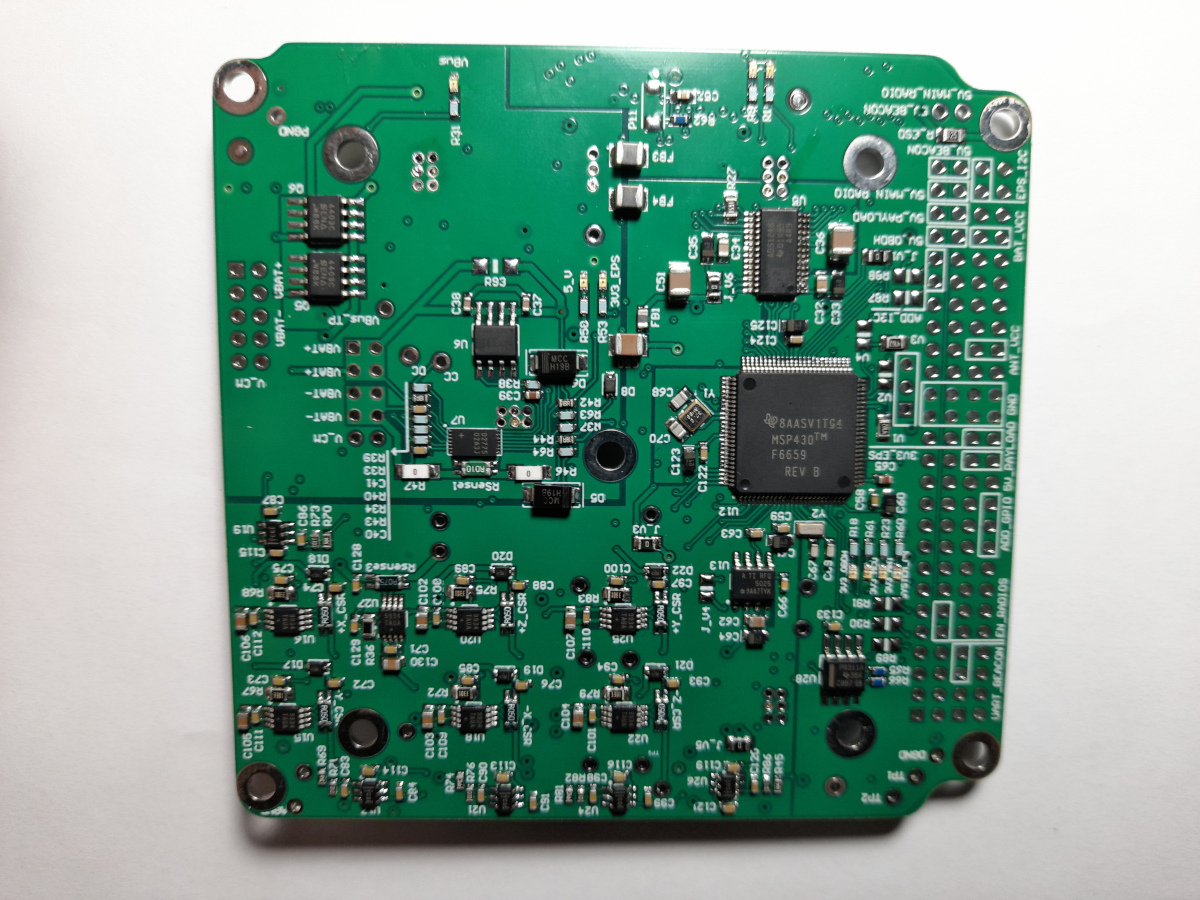
\includegraphics[width=0.75\columnwidth]{figures/v01/eps2-v01-bottom.jpg}
        \caption{Bottom view of the EPS 2.0 v0.1 board.}
        \label{fig:eps2-v01-bottom}
    \end{center}
\end{figure}

\begin{itemize}
    \item \textbf{Test description/Objective}: Inspection of the board, visually and with a multimeter, searching for fabrication and assembly failures.
    \item \textbf{Procedures:} \autoref{tab:visual-inspection}.
    \item \textbf{Material}: None.
    \item \textbf{Results}: The results of this test can be seen in Figures \ref{fig:eps2-v01-top} (top view of the board) and \ref{fig:eps2-v01-bottom} (bottom view of the board).
    \item \textbf{Conclusion}: No major problems were identified on this test, just some labels with typos (all in the PC-104 region) that should be already be corrected for v0.2 and four 4-pin picoblades that were not soldered by the manufacturer due the lack of clearance (differently from the headers and PC-104 which were intentionally removed from the process). This last item might be ignored since the manufacturer used an automated soldering process and the manual placement of these connectors is totally feasible.  
\end{itemize}

\section{Mechanical Inspection}

\begin{itemize}
    \item \textbf{Test description/Objective}: Evaluate if the board has the nominal mechanical specs prior to integration.
    \item \textbf{Procedures:} \autoref{tab:mechanical-inspection}.
    \item \textbf{Material}: None.
    \item \textbf{Results}: The inspection was not performed due to the lack of the proper tools.
    \item \textbf{Conclusion}: Even without the test, the board should not present any problem due to the heritage from the previous models and the good manufacturing quality.
\end{itemize}


\section{Integration Inspection}

\begin{itemize}
    \item \textbf{Test description/Objective}: Analyze the integration accordance prior to the module’s full assembly on the CubeSat.
    \item \textbf{Procedures:} \autoref{tab:integration-inspection}.
    \item \textbf{Material}: None.
    \item \textbf{Results}: Schematic files and pinouts identified in the \autoref{ch:hardware}. 
    \item \textbf{Conclusion}: No problems were identified on this test.
\end{itemize}


\section{Electrical Inspection}

\begin{itemize}
    \item \textbf{Test description/Objective}: Inspect the visually detectable electrical features.
    \item \textbf{Procedures:} \autoref{tab:electrical-inspection}.
    \item \textbf{Material}: None.
    \item \textbf{Results}: The results of this test can be seen in Figures \ref{fig:eps2-v01-top} (top view of the board) and \ref{fig:eps2-v01-bottom} (bottom view of the board).
    \item \textbf{Conclusion}: No problems were identified on this test, components were correctly selected, placed and soldered (except for those already mentioned in the visual inspection).
\end{itemize}


\section{Electrical Testing}

\begin{itemize}
    \item \textbf{Test description/Objective}: Perform basic tests to evaluate the board with nominal operating parameters.
    \item \textbf{Procedures:} \autoref{tab:electrical-testing}.
    \item \textbf{Material}:
        \begin{itemize}
            \item Multimeter Fluke 179
            \item Keysight N6705B DC Power Analyzer
        \end{itemize}
    \item \textbf{Results}: Results reported with the following images: \ref{fig:electrical-test-setup}, \ref{fig:power-consumption}, \ref{fig:regulator-payload}, \ref{fig:regulator-antenna}, \ref{fig:regulator-radio0}, \ref{fig:regulator-radio1}, \ref{fig:regulator-obdh} and \ref{fig:regulator-epsttc}. 
    \item \textbf{Conclusion}: The boards power-up as expected and present stable power consumption. The power outputs (step-down regulators) underperform with nominal or slightly higher load parameters. The issue might be related to poor sizing of passive components required for the regulators. This problem \textbf{must} be solved for the next version (it is expected to be performed minor changes in components values).  
\end{itemize}

\begin{figure}[!htb]
    \begin{center}
        \subfigure[Test setup for power characterization.\label{fig:electrical-test-tools}]{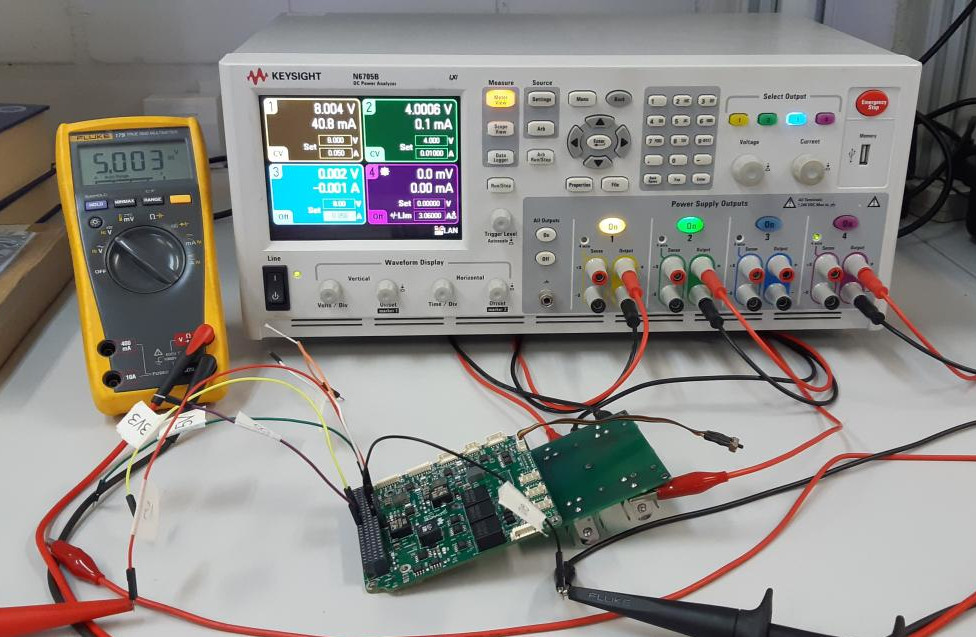
\includegraphics[height=0.28\textheight]{figures/v01/electrical-test-tools.jpg}}
        ~
        \subfigure[Board connectors and harness used during the tests.\label{fig:electrical-test-board}]{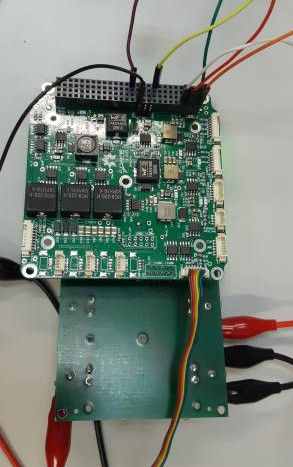
\includegraphics[height=0.28\textheight]{figures/v01/electrical-test-board.jpg}}
        \caption{Electrical test setup of the power-up sequence and output power supply channels.}
        \label{fig:electrical-test-setup}
    \end{center}
\end{figure}

\begin{figure}[!ht]
    \begin{center}
        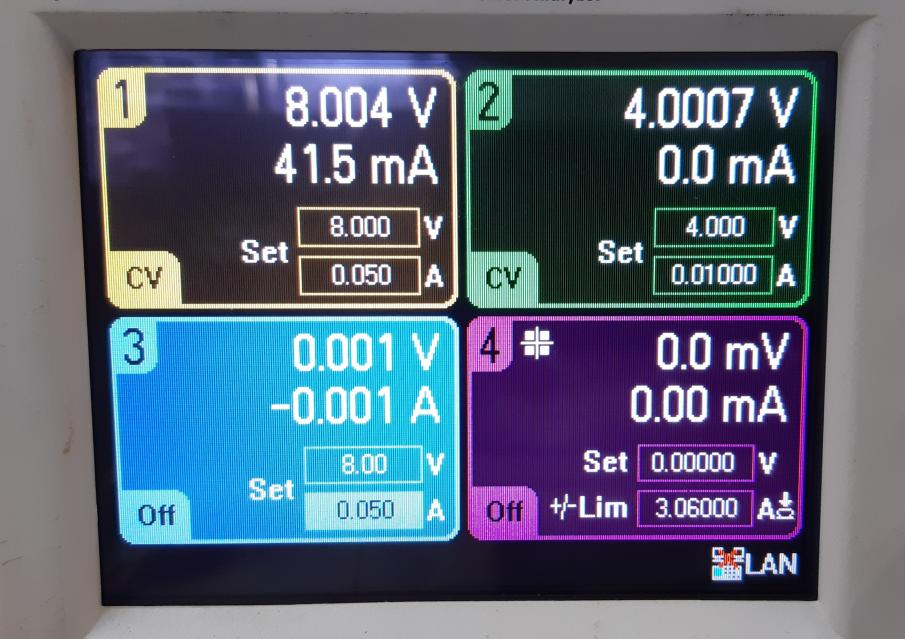
\includegraphics[width=\columnwidth]{figures/v01/power-consumption.jpg}
        \caption{Power consumption during standby with any intensive firmware task.}
        \label{fig:power-consumption}
    \end{center}
\end{figure}

\begin{figure}[!htb]
    \begin{center}
        \subfigure[Load: 0mA.\label{fig:regulator-payload-0mA}]{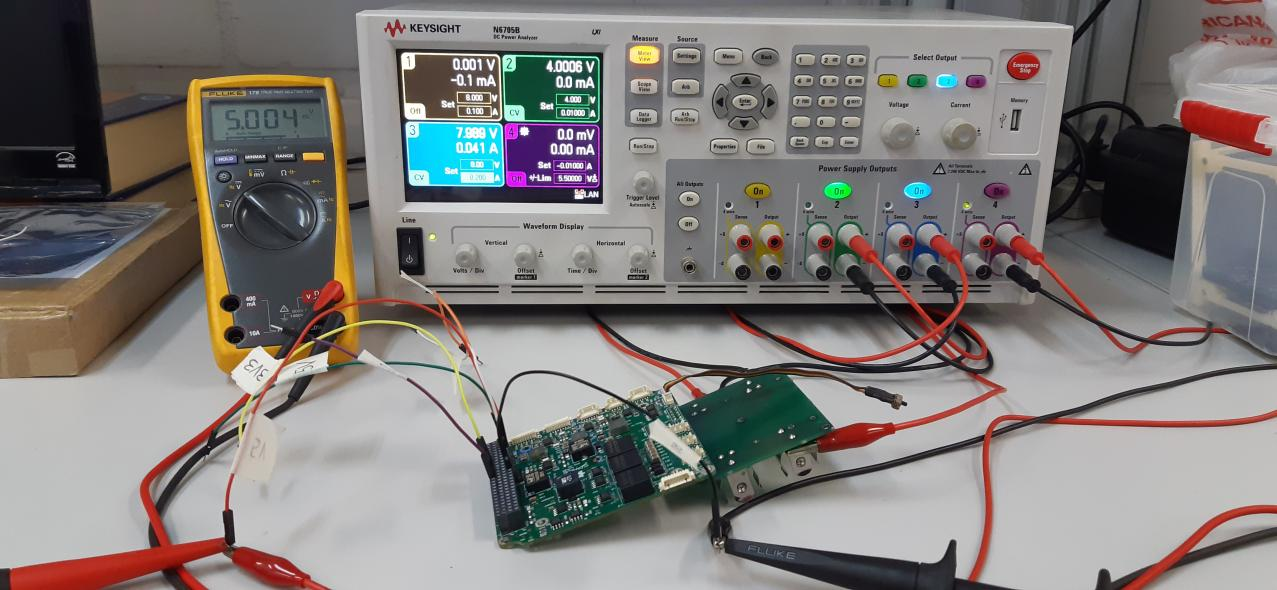
\includegraphics[height=0.19\textheight]{figures/v01/regulator-payload-0mA.jpg}}
        ~
        \subfigure[Load: 500mA.\label{fig:regulator-payload-500mA}]{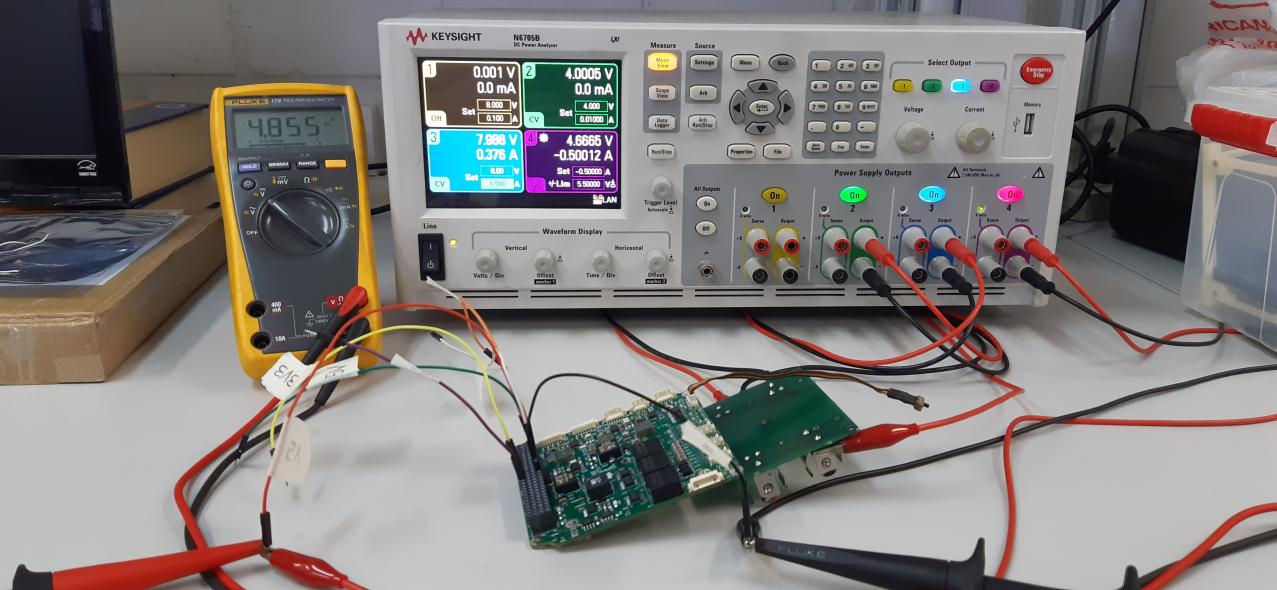
\includegraphics[height=0.19\textheight]{figures/v01/regulator-payload-500mA.jpg}}
        ~
        \subfigure[Load: 1000mA.\label{fig:regulator-payload-1000mA}]{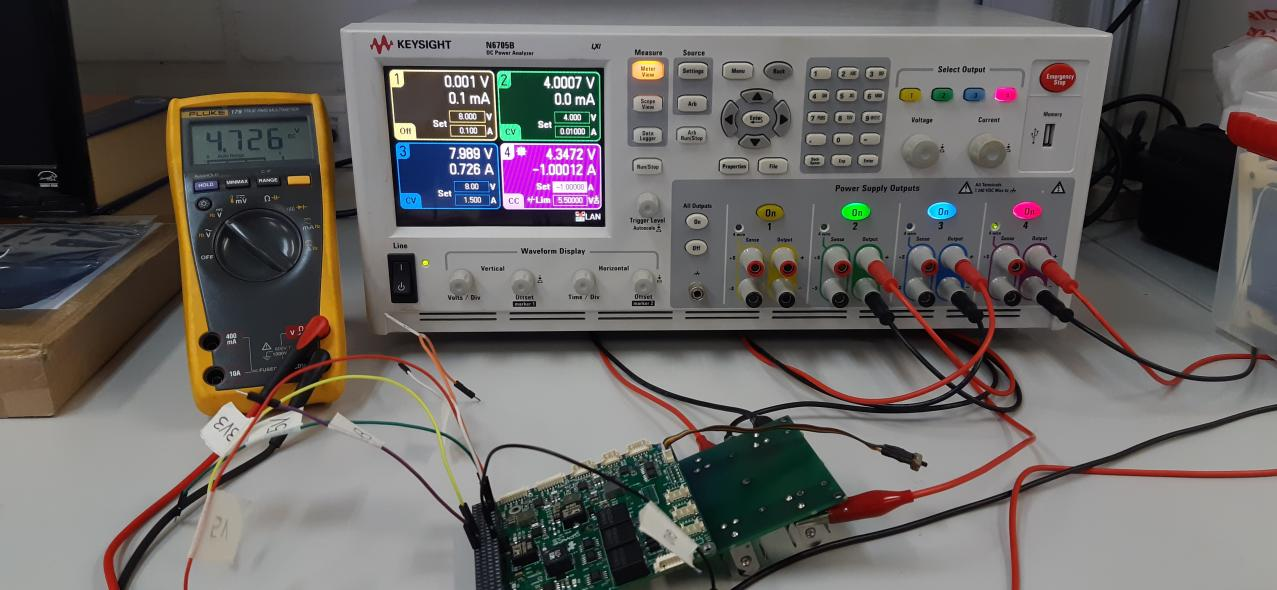
\includegraphics[height=0.19\textheight]{figures/v01/regulator-payload-1000mA.jpg}}
        ~
        \subfigure[Load: 1500mA.\label{fig:regulator-payload-1500mA}]{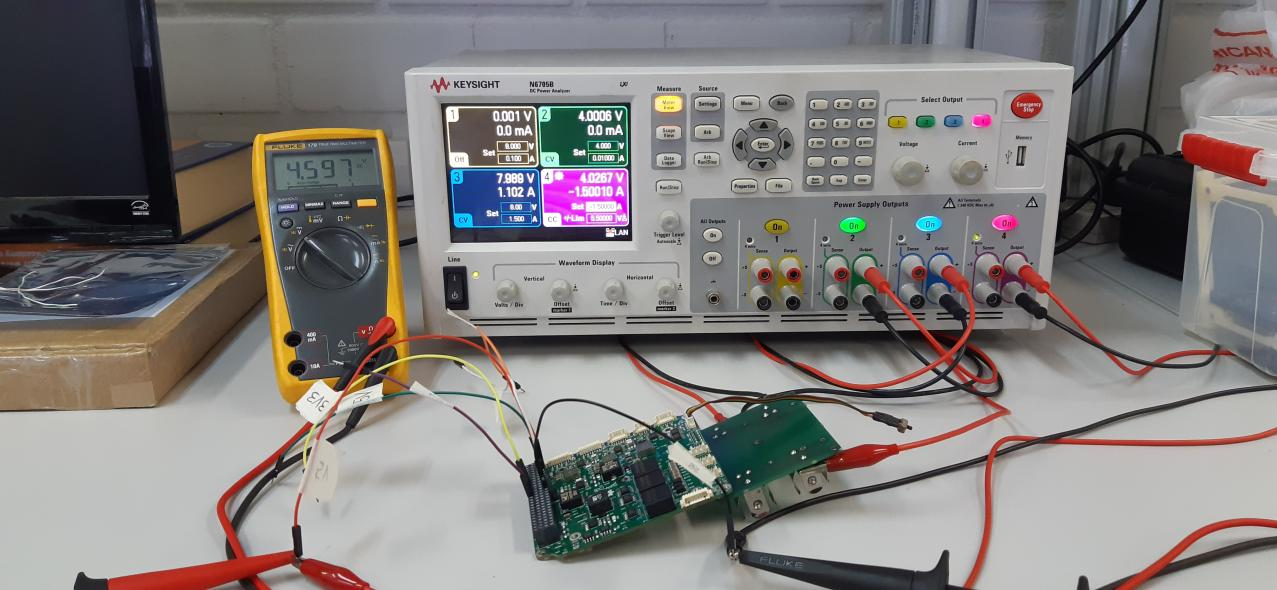
\includegraphics[height=0.19\textheight]{figures/v01/regulator-payload-1500mA.jpg}}
        
        \caption{Payload step-down regulator power characterization.}
        \label{fig:regulator-payload}
    \end{center}
\end{figure}

\begin{figure}[!htb]
    \begin{center}
        \subfigure[Load: 0mA.\label{fig:regulator-antenna-0mA}]{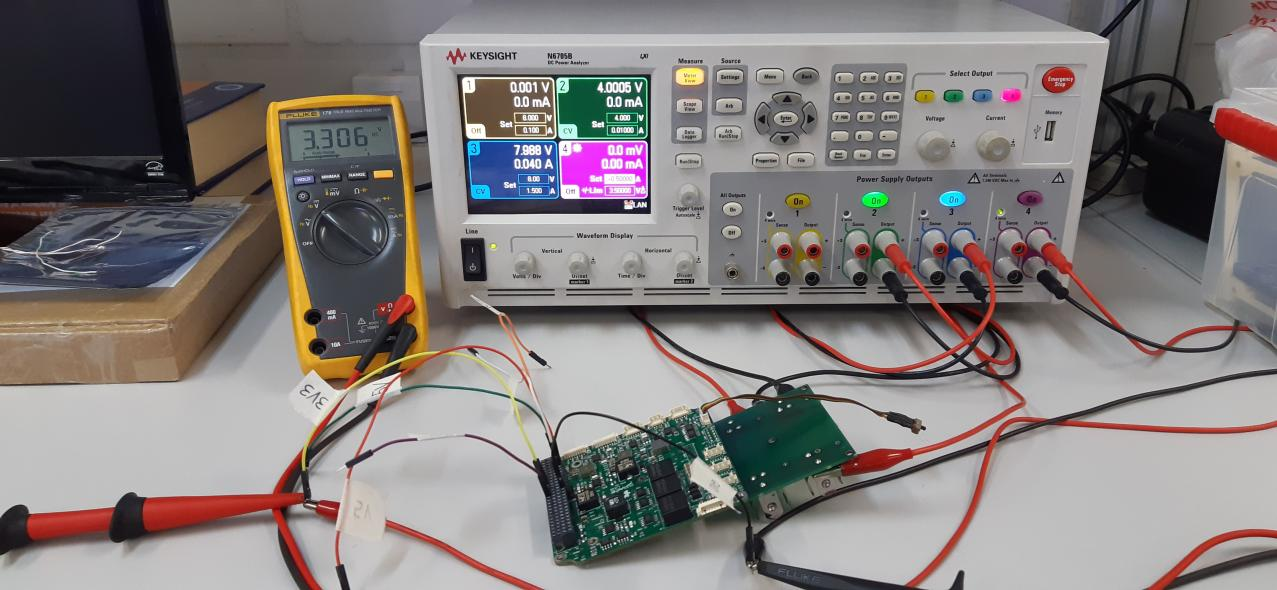
\includegraphics[height=0.19\textheight]{figures/v01/regulator-antenna-0mA.jpg}}
        ~
        \subfigure[Load: 500mA.\label{fig:regulator-antenna-500mA}]{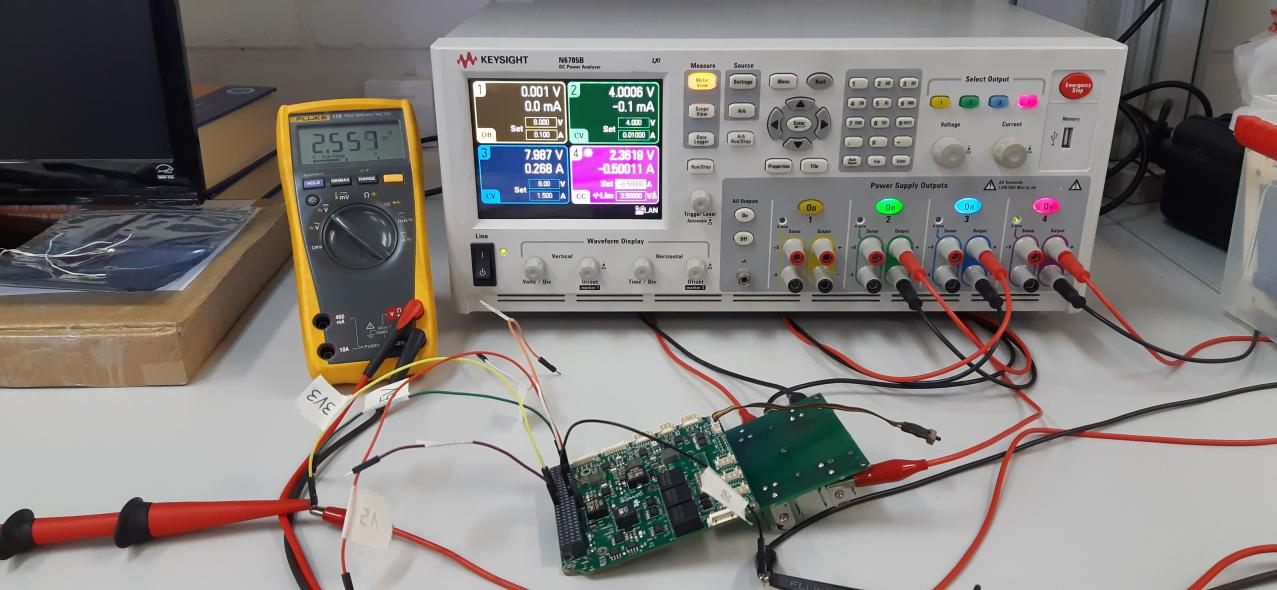
\includegraphics[height=0.19\textheight]{figures/v01/regulator-antenna-500mA.jpg}}
        ~
        \subfigure[Load: 1000mA.\label{fig:regulator-antenna-1000mA}]{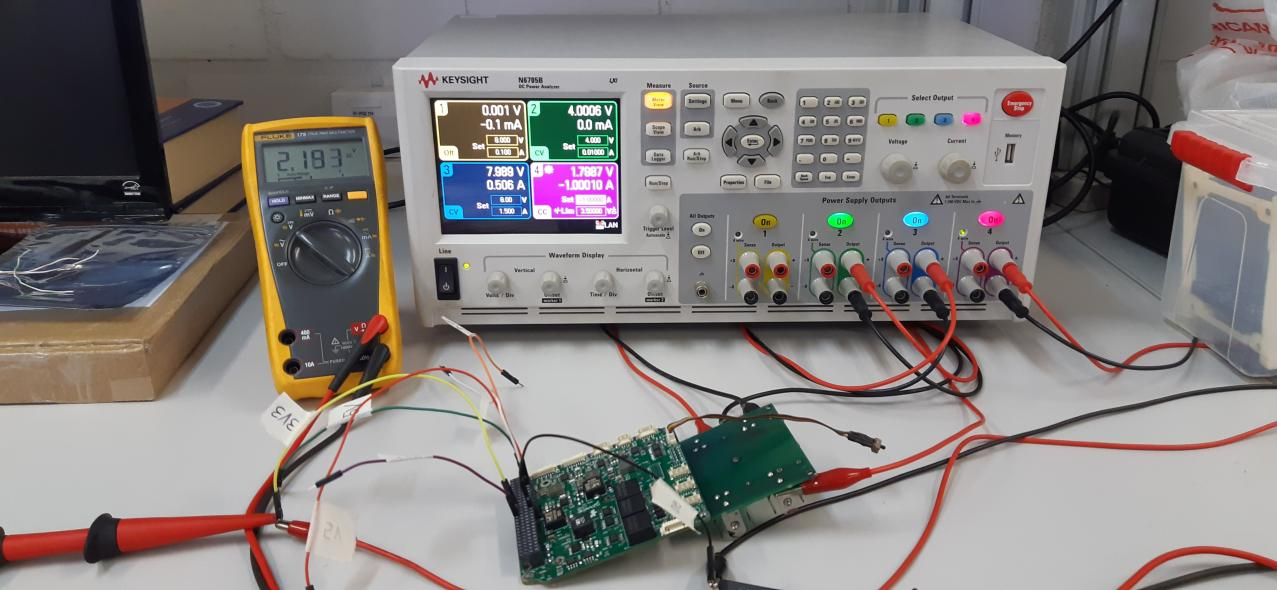
\includegraphics[height=0.19\textheight]{figures/v01/regulator-antenna-1000mA.jpg}}
        ~
        \subfigure[Load: 1500mA.\label{fig:regulator-antenna-1500mA}]{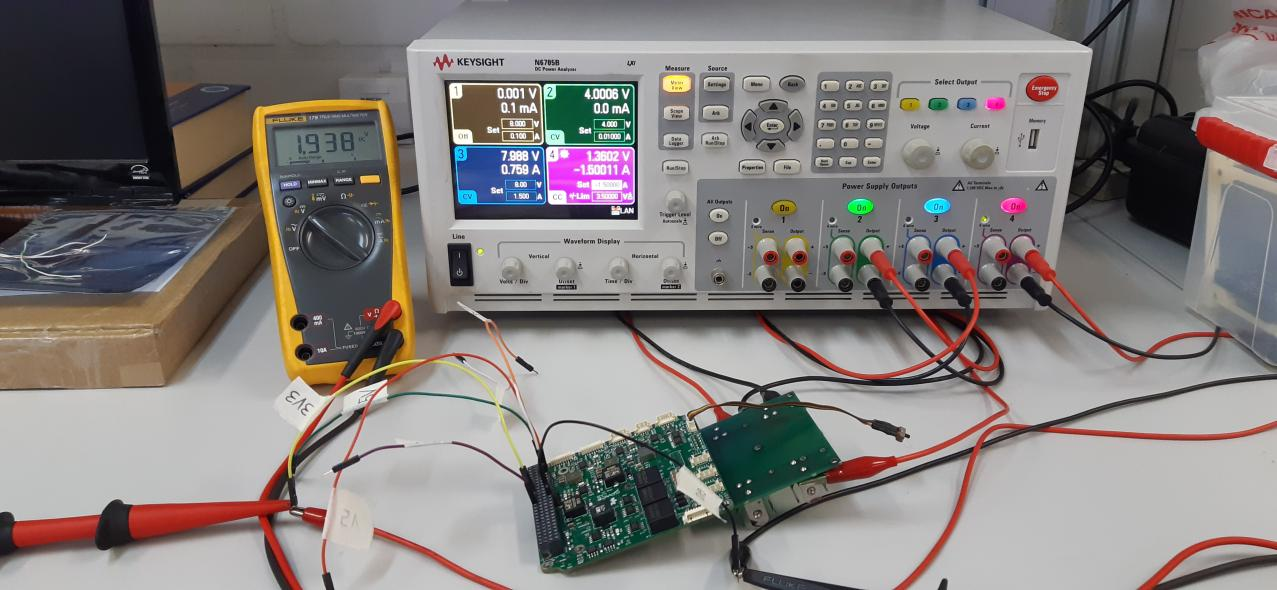
\includegraphics[height=0.19\textheight]{figures/v01/regulator-antenna-1500mA.jpg}}
        
        \caption{Antenna step-down regulator power characterization.}
        \label{fig:regulator-antenna}
    \end{center}
\end{figure}

\begin{figure}[!htb]
    \begin{center}
        \subfigure[Load: 0mA.\label{fig:regulator-radio0-0mA}]{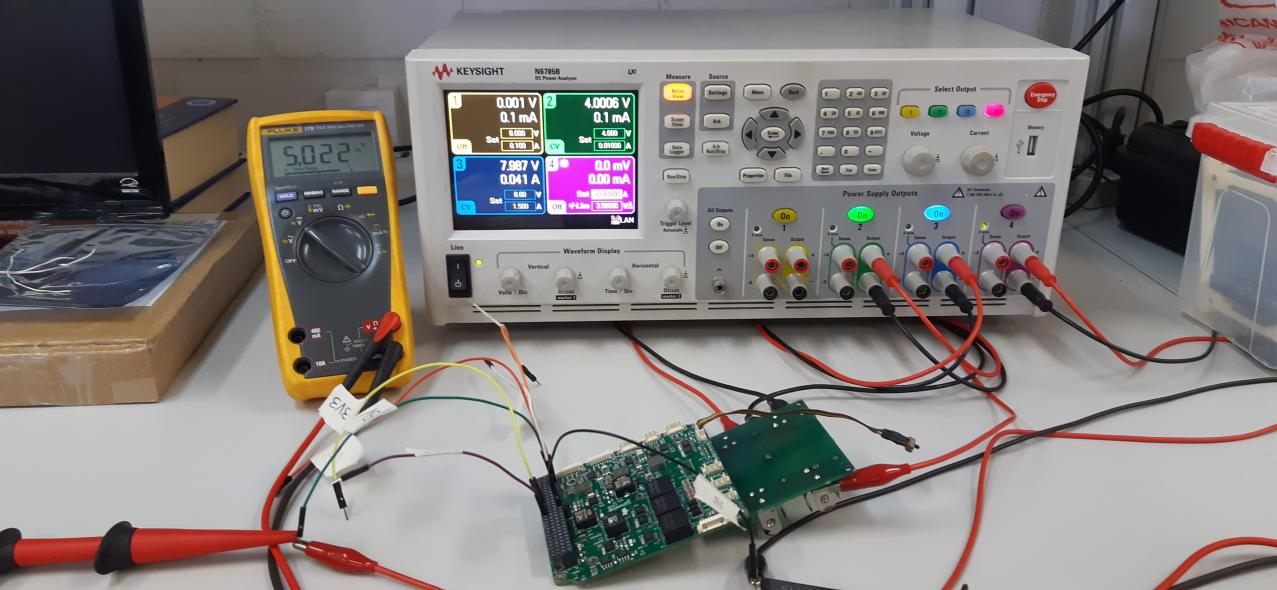
\includegraphics[height=0.19\textheight]{figures/v01/regulator-radio0-0mA.jpg}}
        ~
        \subfigure[Load: 500mA.\label{fig:regulator-radio0-500mA}]{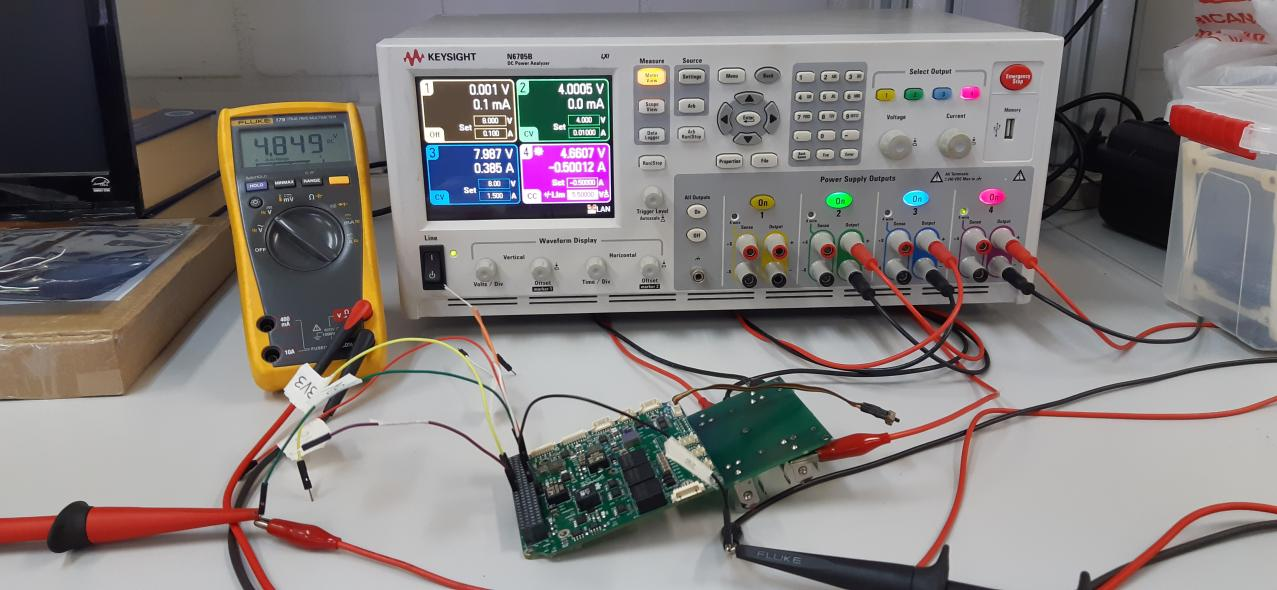
\includegraphics[height=0.19\textheight]{figures/v01/regulator-radio0-500mA.jpg}}
        ~
        \subfigure[Load: 1000mA.\label{fig:regulator-radio0-1000mA}]{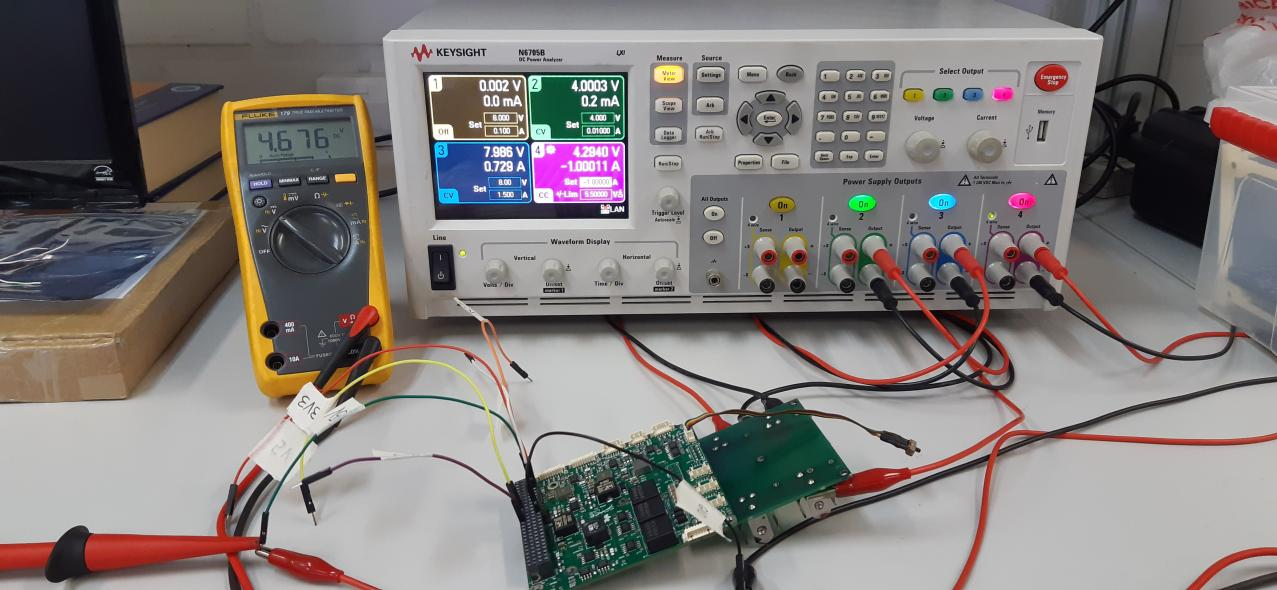
\includegraphics[height=0.19\textheight]{figures/v01/regulator-radio0-1000mA.jpg}}
        ~
        \subfigure[Load: 1500mA.\label{fig:regulator-radio0-1500mA}]{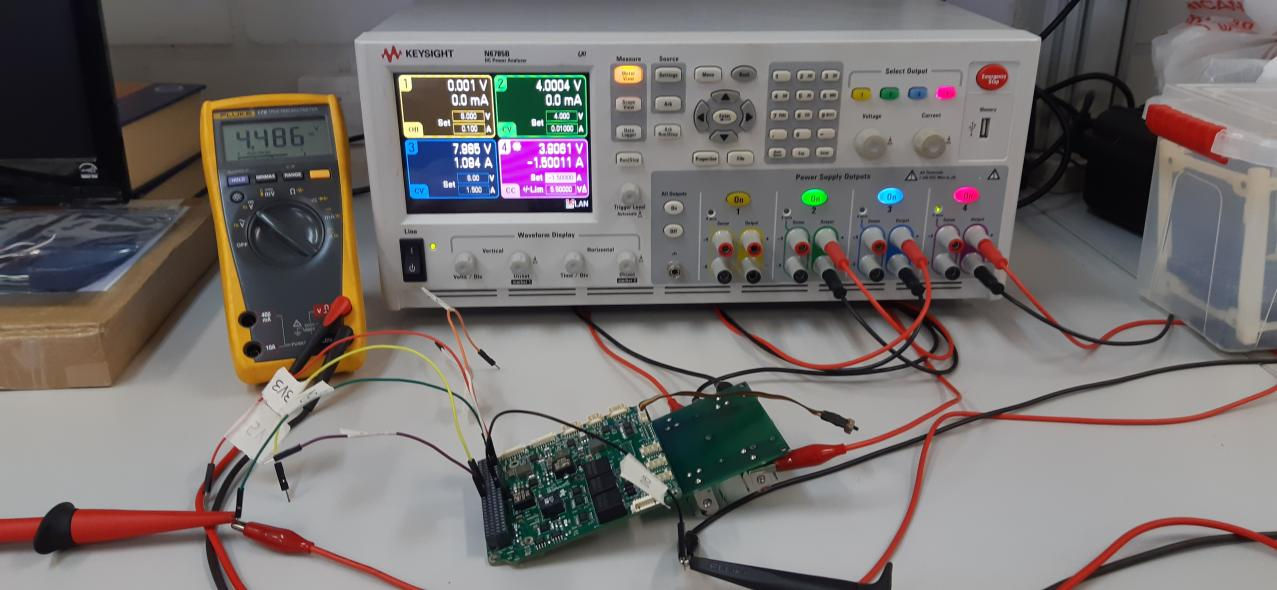
\includegraphics[height=0.19\textheight]{figures/v01/regulator-radio0-1500mA.jpg}}
        
        \caption{Radio 0 step-down regulator power characterization.}
        \label{fig:regulator-radio0}
    \end{center}
\end{figure}

\begin{figure}[!htb]
    \begin{center}
        \subfigure[Load: 0mA.\label{fig:regulator-radio1-0mA}]{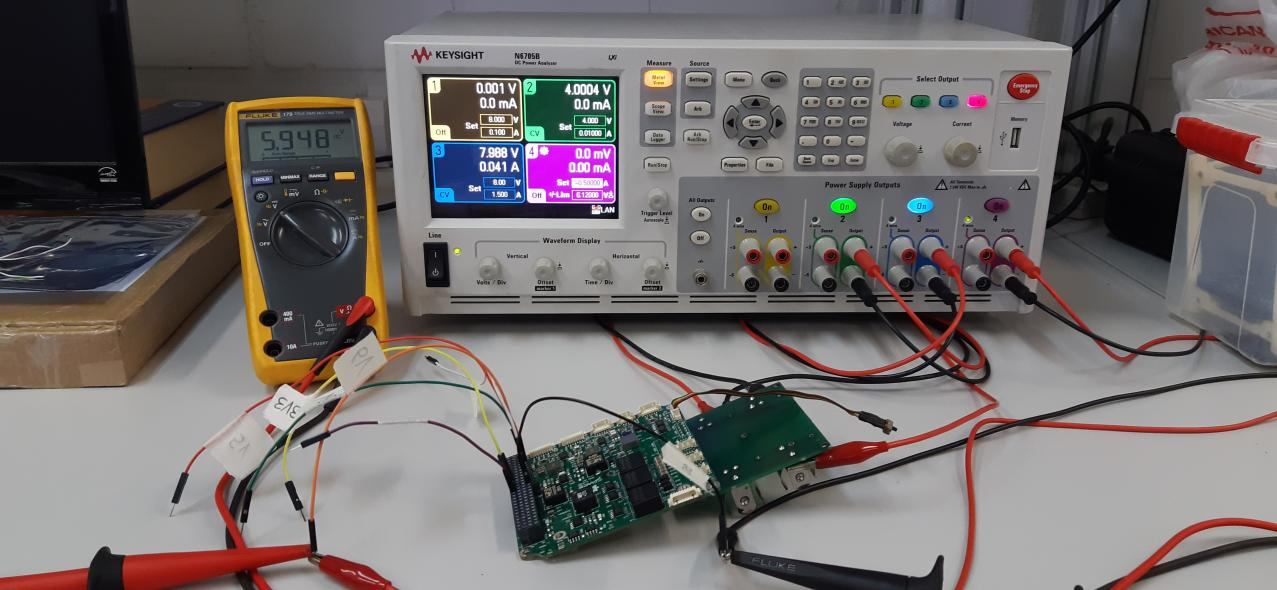
\includegraphics[height=0.19\textheight]{figures/v01/regulator-radio1-0mA.jpg}}
        ~
        \subfigure[Load: 500mA.\label{fig:regulator-radio1-500mA}]{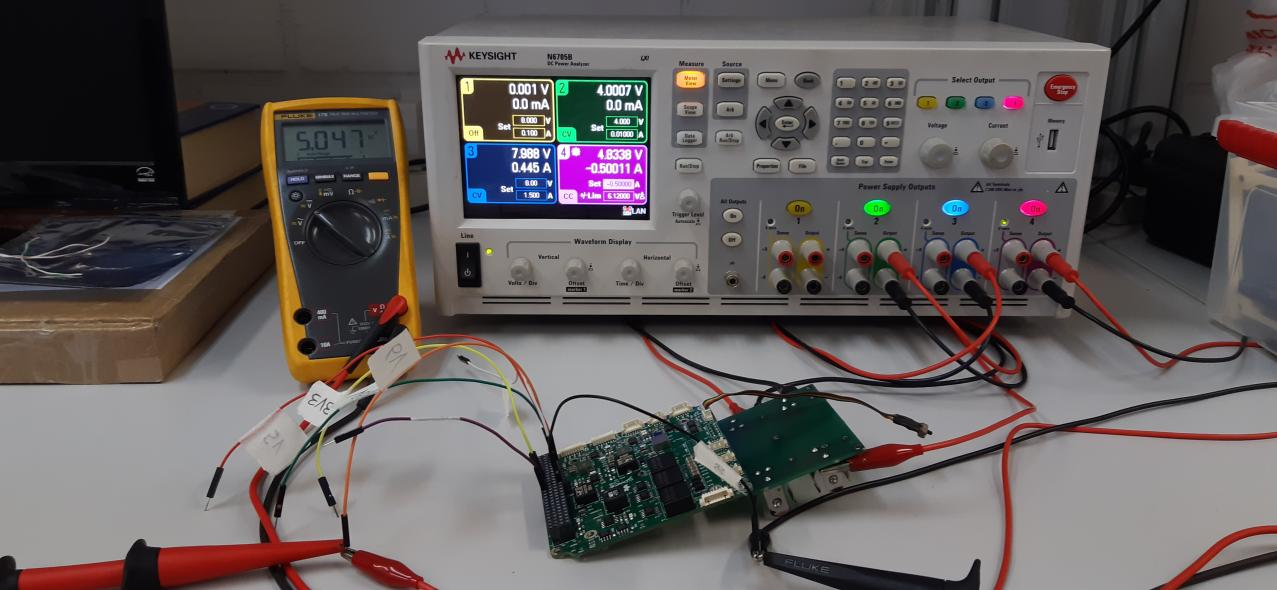
\includegraphics[height=0.19\textheight]{figures/v01/regulator-radio1-500mA.jpg}}
        ~
        \subfigure[Load: 1000mA.\label{fig:regulator-radio1-1000mA}]{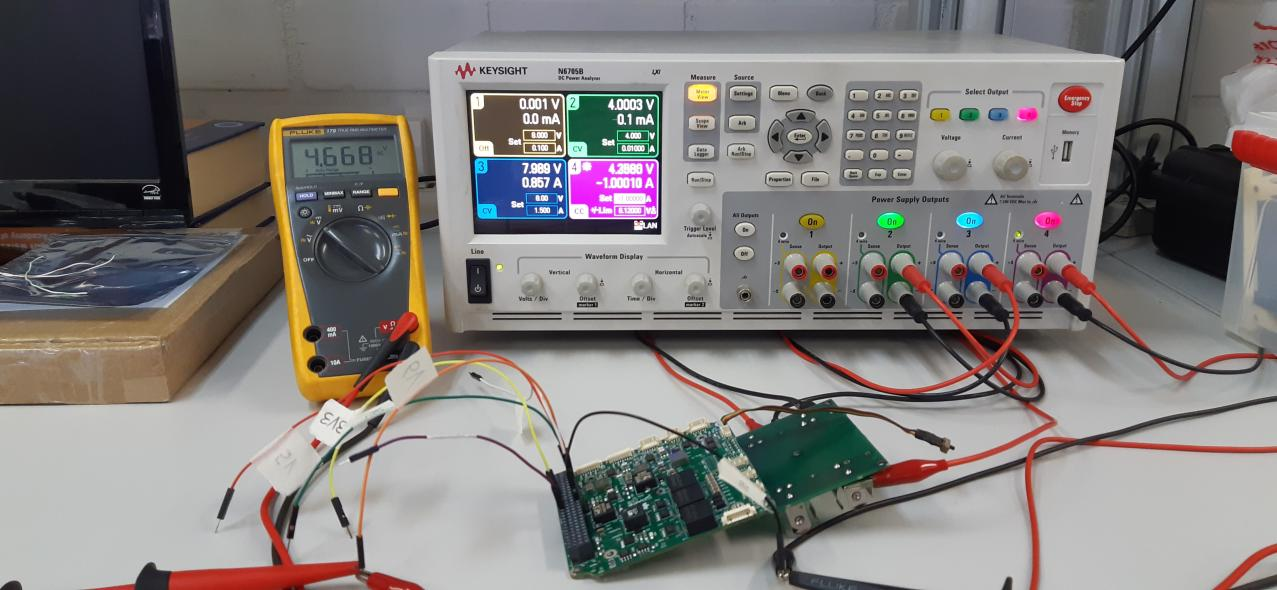
\includegraphics[height=0.19\textheight]{figures/v01/regulator-radio1-1000mA.jpg}}
        ~
        \subfigure[Load: 1500mA.\label{fig:regulator-radio1-1500mA}]{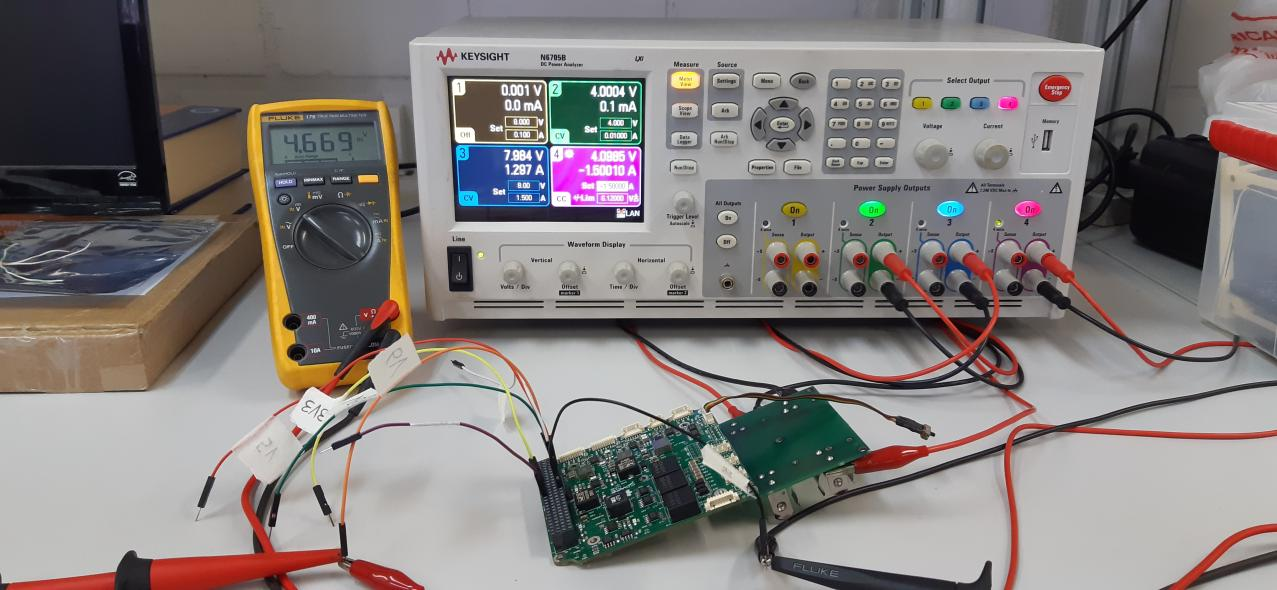
\includegraphics[height=0.19\textheight]{figures/v01/regulator-radio1-1500mA.jpg}}
        
        \caption{Radio 1 step-down regulator power characterization.}
        \label{fig:regulator-radio1}
    \end{center}
\end{figure}

\begin{figure}[!htb]
    \begin{center}
        \subfigure[Load: 0mA.\label{fig:regulator-obdh-0mA}]{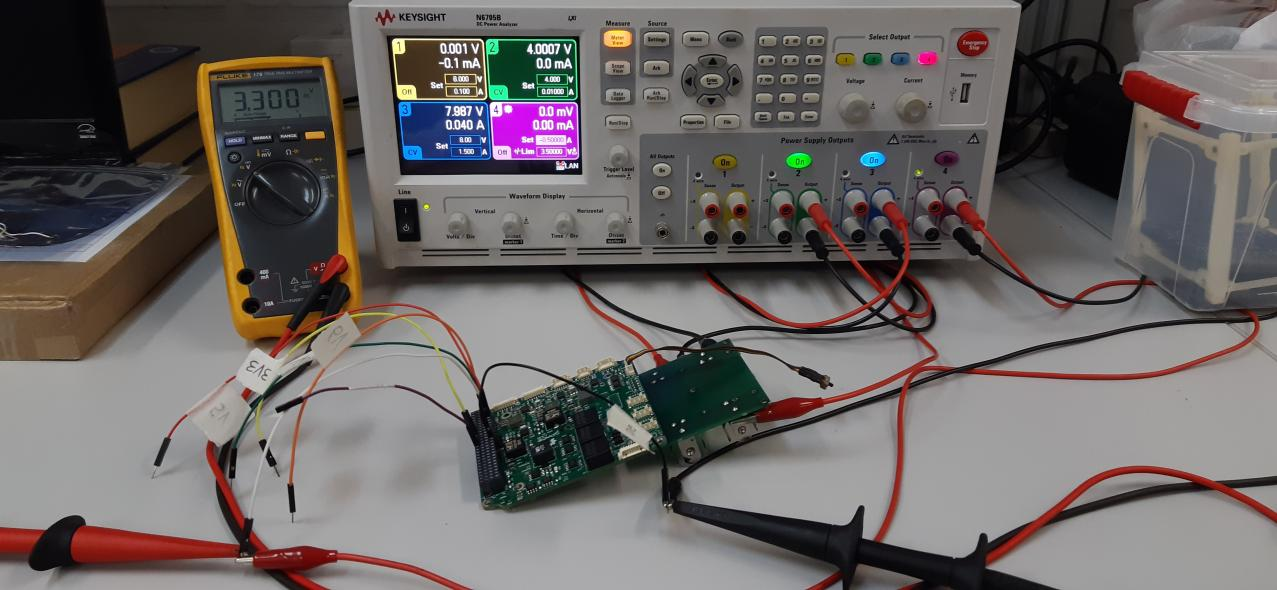
\includegraphics[height=0.19\textheight]{figures/v01/regulator-obdh-0mA.jpg}}
        ~
        \subfigure[Load: 500mA.\label{fig:regulator-obdh-100mA}]{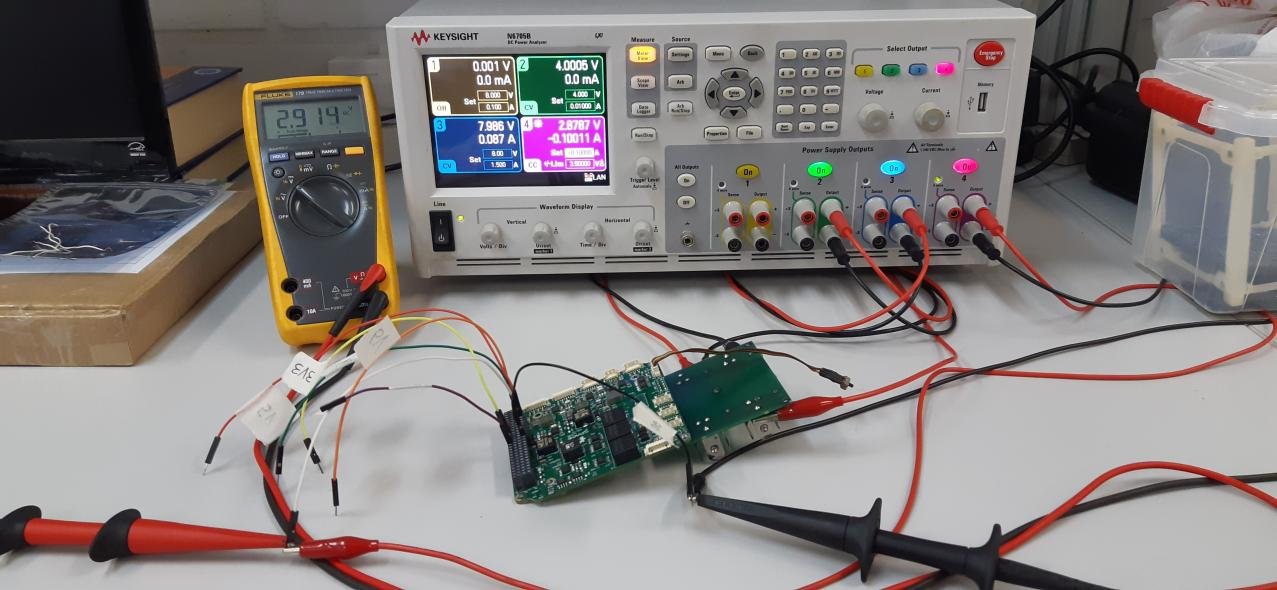
\includegraphics[height=0.19\textheight]{figures/v01/regulator-obdh-100mA.jpg}}
        ~
        \subfigure[Load: 1000mA.\label{fig:regulator-obdh-200mA}]{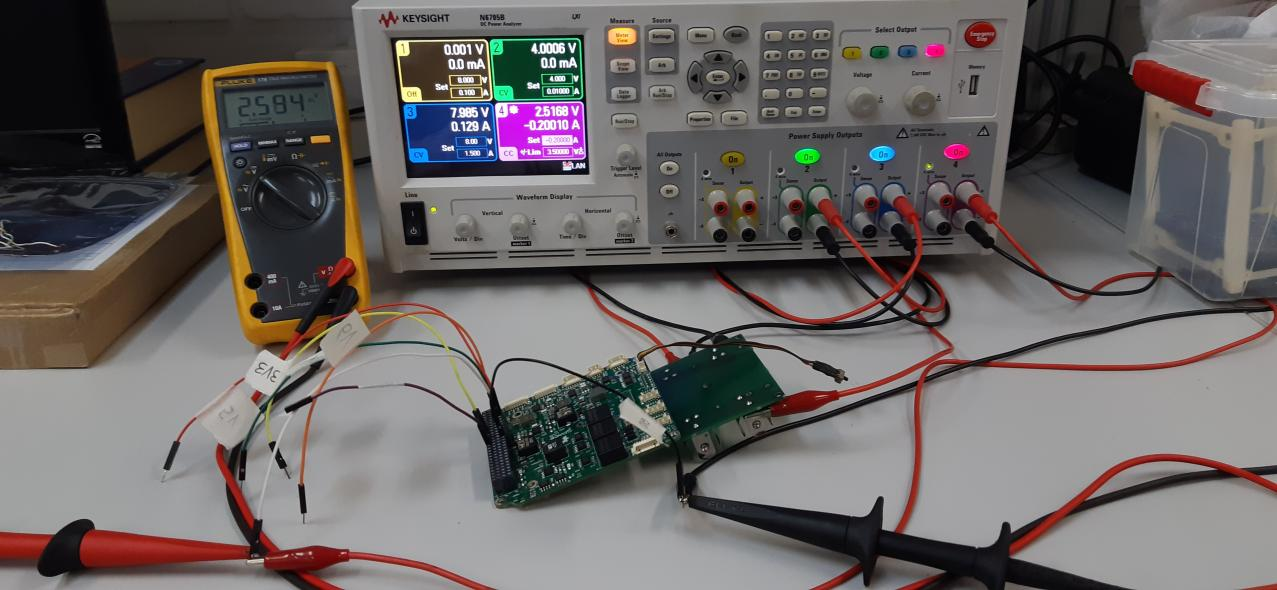
\includegraphics[height=0.19\textheight]{figures/v01/regulator-obdh-200mA.jpg}}
        ~
        \subfigure[Load: 1500mA.\label{fig:regulator-obdh-500mA}]{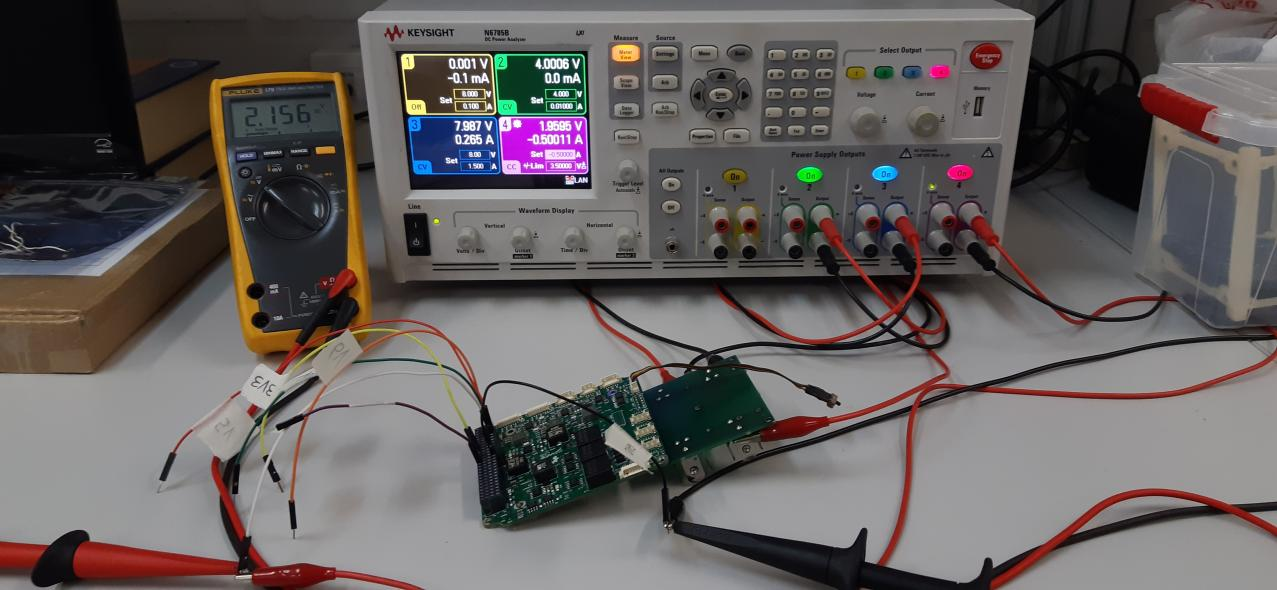
\includegraphics[height=0.19\textheight]{figures/v01/regulator-obdh-500mA.jpg}}
        
        \caption{OBDH step-down regulator power characterization.}
        \label{fig:regulator-obdh}
    \end{center}
\end{figure}

\begin{figure}[!htb]
    \begin{center}
        \subfigure[Load: 0mA.\label{fig:regulator-epsttc-0mA}]{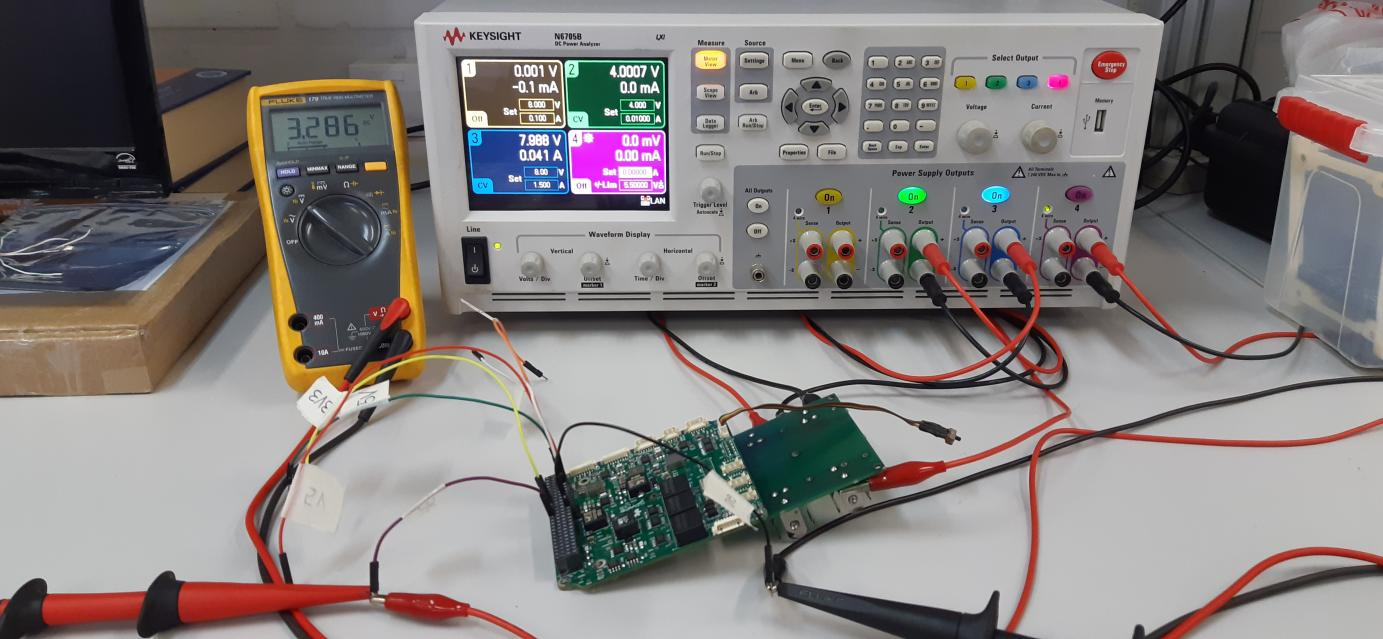
\includegraphics[height=0.19\textheight]{figures/v01/regulator-epsttc-0mA.jpg}}
        ~
        \subfigure[Load: 500mA.\label{fig:regulator-epsttc-500mA}]{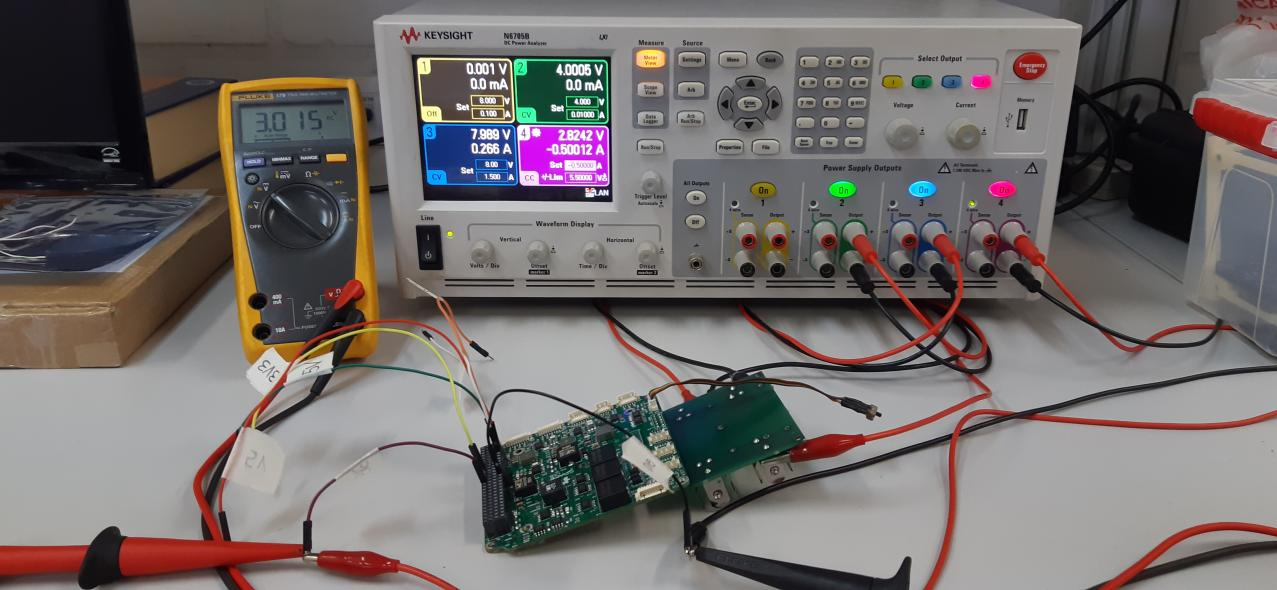
\includegraphics[height=0.19\textheight]{figures/v01/regulator-epsttc-500mA.jpg}}
        ~
        \subfigure[Load: 1000mA.\label{fig:regulator-epsttc-1000mA}]{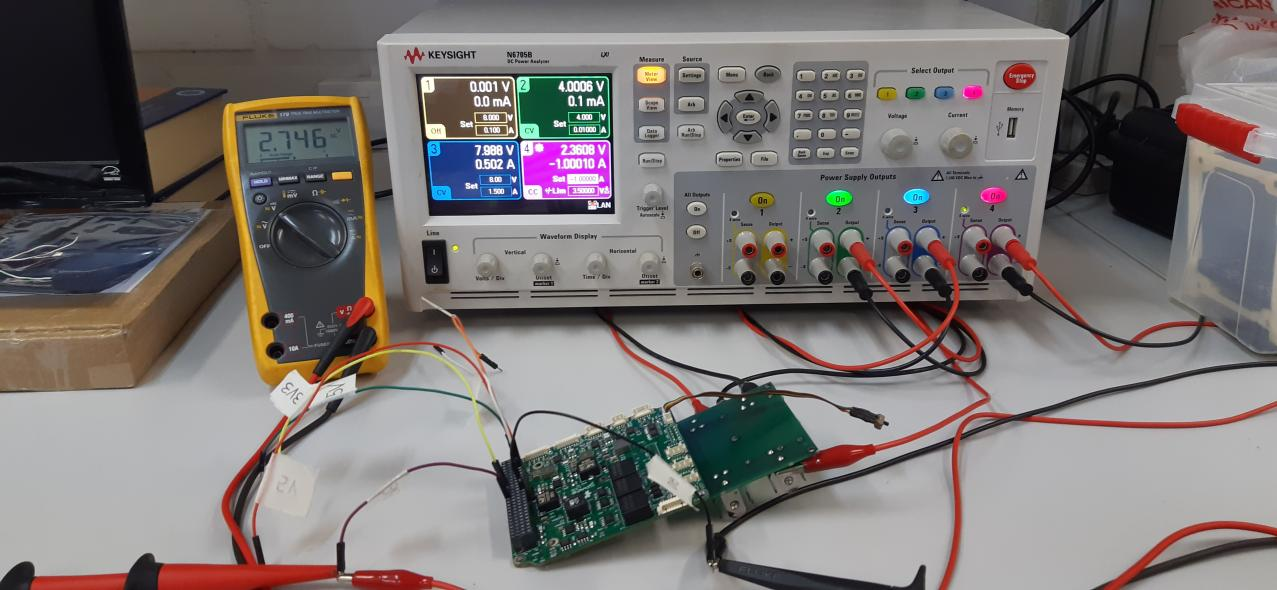
\includegraphics[height=0.19\textheight]{figures/v01/regulator-epsttc-1000mA.jpg}}

        \caption{EPS/TTC step-down regulator power characterization.}
        \label{fig:regulator-epsttc}
    \end{center}
\end{figure}
 
 \newpage

\section{Functional Testing}

\subsection{Firmware Programming}

\begin{itemize}
    \item \textbf{Test description/Objective}: Evaluate the board behavior under a firmware programming sequence.
    \item \textbf{Material}:
        \begin{itemize}
            \item Code Composer Studio v10.0.0
            \item MSP-FET Flash Emulation Tool
            \item USB-UART converter
            \item PuTTy
        \end{itemize}
    \item \textbf{Results}: The results of this are available in \autoref{fig:log-first-boot}, where the log messages of the first boot of the board can be seen.
    \item \textbf{Conclusion}: Major problems were identified on this test, but it was expected since the available firmware version was at early stages of refactoring and development.
\end{itemize}

\begin{figure}[!htb]
    \begin{center}
        \subfigure[Board connections using the MSP-FET and USB-UART converter.\label{fig:setup-first-boot}]{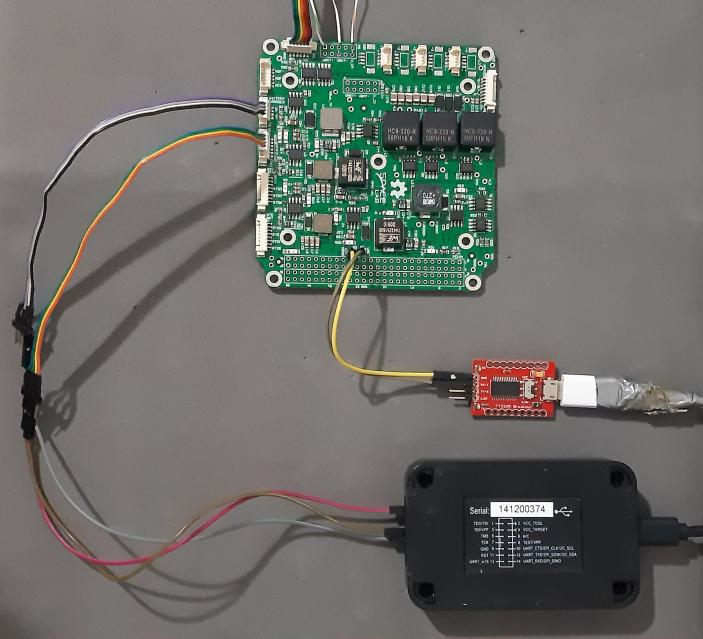
\includegraphics[height=0.2\textheight]{figures/v01/setup-first-boot.jpg}}
        ~
        \subfigure[Pin connections using the MSP-FET and USB-UART converter.\label{fig:electrical-test-board}]{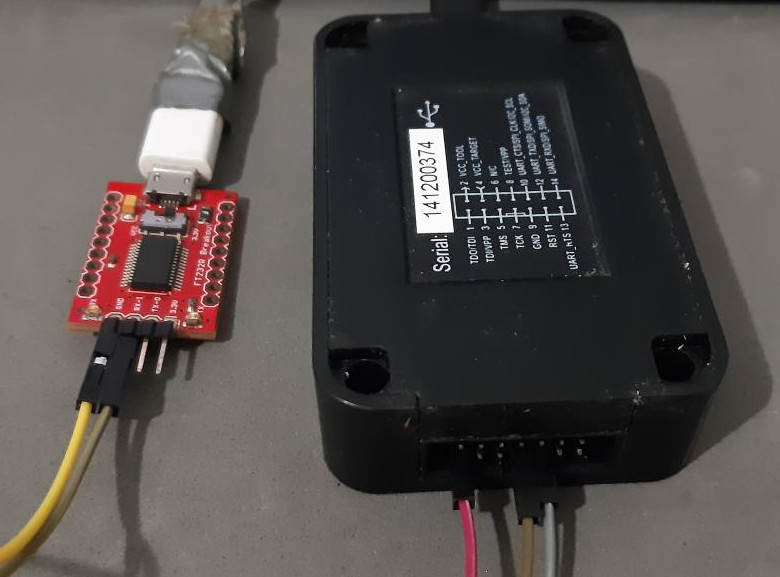
\includegraphics[height=0.2\textheight]{figures/v01/tools-first-boot.jpg}}
        \caption{Setup used for the first firmware boot}
        \label{fig:setup-first-boot}
    \end{center}
\end{figure}

\begin{figure}[!ht]
    \begin{center}
        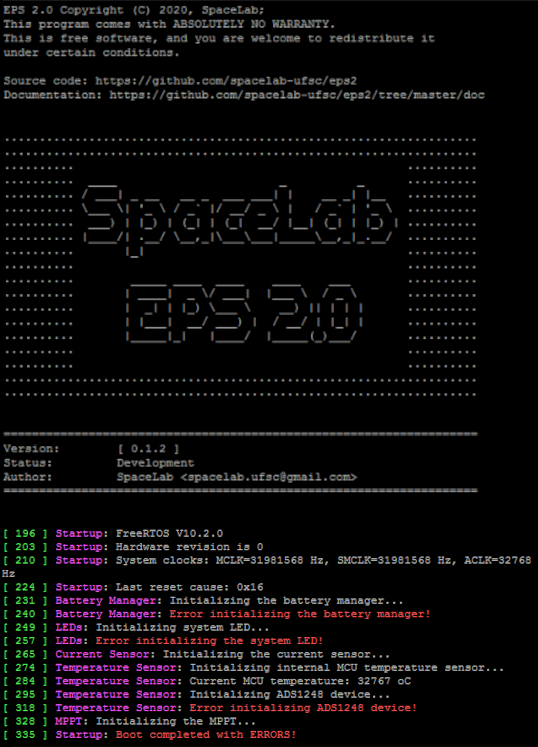
\includegraphics[width=0.4\columnwidth]{figures/v01/log-first-boot.png}
        \caption{Log messages during the first boot.}
        \label{fig:log-first-boot}
    \end{center}
\end{figure}

%\subsection{Communication Buses}
%
%\begin{itemize}
%    \item \textbf{Test description/Objective}: Test the communication busses of the board, as listed below:
%        \begin{itemize}
%            \item I$^{2}$C Port 0
%            \item I$^{2}$C Port 1
%            \item I$^{2}$C Port 2
%        \end{itemize}
%    \item \textbf{Material}:
%        \begin{itemize}
%            \item Saleae Logic Analyzer (24 MHz, 8 channels)
%            \item Saleae Logic software (v1.2.18)
%            \item MSP-FET Flash Emulation Tool
%        \end{itemize}
%    \item \textbf{Results}: The results of this test can be seen in Figures \ref{fig:test-i2c-0}, \ref{fig:test-i2c-1} and \ref{fig:test-i2c-2}.
%    \item \textbf{Conclusion:} No problems were identified on this test, all buses are working as expected.
%\end{itemize}
%
%\begin{figure}[!htb]
%    \begin{center}
%        \subfigure[Connections of the I$^{2}$C port 0 test.\label{fig:connections-i2c-0}]{\includegraphics[height=0.22\textheight]{figures/v05/test-i2c-0.jpg}}
%        ~
%        \subfigure[Waveforms of the I$^{2}$C port 0 test.\label{fig:waveform-i2c-0}]{\includegraphics[height=0.22\textheight]{figures/v05/waveform-i2c-0.png}}
%        \caption{I$^{2}$C port 0 test.}
%        \label{fig:test-i2c-0}
%    \end{center}
%\end{figure}
%
%
%
%\begin{figure}[!htb]
%    \begin{center}
%        \subfigure[Connections of the I$^{2}$C port 1 test.\label{fig:connections-i2c-1}]{\includegraphics[height=0.22\textheight]{figures/v05/test-i2c-1.jpg}}
%        ~
%        \subfigure[Waveforms of the I$^{2}$C port 1 test.\label{fig:waveform-i2c-1}]{\includegraphics[height=0.22\textheight]{figures/v05/waveform-i2c-1.png}}
%        \caption{I$^{2}$C port 1 test.}
%        \label{fig:test-i2c-1}
%    \end{center}
%\end{figure}
%
%
%
%\begin{figure}[!htb]
%    \begin{center}
%        \subfigure[Connections of the I$^{2}$C port 2 test.\label{fig:connections-i2c-2}]{\includegraphics[height=0.22\textheight]{figures/v05/test-i2c-2.jpg}}
%        ~
%        \subfigure[Waveforms of the I$^{2}$C port 2 test.\label{fig:waveform-i2c-2}]{\includegraphics[height=0.22\textheight]{figures/v05/waveform-i2c-2.png}}
%        \caption{I$^{2}$C port 2 test.}
%        \label{fig:test-i2c-2}
%    \end{center}
%\end{figure}
%
%\subsection{Sensors}
%
%\subsection{Input Voltage}
%
%\begin{itemize}
%    \item \textbf{Test description/Objective}: .
%    \item \textbf{Material}:
%        \begin{itemize}
%            \item Code Composer Studio v9.3.0
%            \item MSP-FET Flash Emulation Tool
%            \item USB-UART converter
%            \item Screen (Linux software)
%        \end{itemize}
%    \item \textbf{Results}: .
%    \item \textbf{Conclusion:} .
%\end{itemize}
%
%\subsection{Input Current}
%
%\begin{itemize}
%    \item \textbf{Test description/Objective}: .
%    \item \textbf{Material}:
%        \begin{itemize}
%            \item Code Composer Studio v9.3.0
%            \item MSP-FET Flash Emulation Tool
%            \item USB-UART converter
%            \item Screen (Linux software)
%        \end{itemize}
%    \item \textbf{Results}: .
%    \item \textbf{Conclusion:} .
%\end{itemize}
%
%\begin{figure}[!htb]
%    \begin{center}
%        \subfigure[Current sensing circuit.\label{fig:current-sensing-circuit-v05}]{\includegraphics[width=0.8\textwidth]{figures/v05/current-sensor-circuit.png}}
%
%        \subfigure[MAX9934 pinout.\label{fig:max9934-pinout}]{\includegraphics[width=0.4\textwidth]{figures/v05/max9934-top-view.png}}
%        ~
%        \subfigure[Current sensing layout (bottom layer).\label{fig:}]{\includegraphics[width=0.4\textwidth]{figures/v05/current-sensor-layout.png}}
%        \caption{.}
%        \label{fig:current-sensing-error-v05}
%    \end{center}
%\end{figure}
%
%\begin{figure}[!ht]
%    \begin{center}
%        \includegraphics[width=0.6\columnwidth]{figures/v05/max9934-fix.jpg}
%        \caption{Current sensor fix.}
%        \label{fig:current-sensor-fix}
%    \end{center}
%\end{figure}
%
%\begin{figure}[!ht]
%    \begin{center}
%        \includegraphics[width=0.7\columnwidth]{figures/v05/log-current-sensor.png}
%        \caption{Log messages with the read values from the current sensor.}
%        \label{fig:log-current-sensor}
%    \end{center}
%\end{figure}
%
%\subsection{Peripherals}
%
%\subsection{NOR Flash Memory}
%
%\begin{itemize}
%    \item \textbf{Test description/Objective}: Test the functionality of the NOR flash memory by verifying the device ID register of the IC.
%    \item \textbf{Material}:
%        \begin{itemize}
%            \item Saleae Logic Analyzer (24 MHz, 8 channels)
%            \item Saleae Logic software (v1.2.18)
%            \item MSP-FET Flash Emulation Tool
%        \end{itemize}
%    \item \textbf{Results}: The results of this test can be seen in \autoref{fig:test-nor-memory}.
%    \item \textbf{Conclusion:} No problems were identified on this test, as can be seen in \autoref{fig:waveform-spi-mem}, the device ID register was read as expected.
%\end{itemize}
%
%\begin{figure}[!htb]
%    \begin{center}
%        \subfigure[Connections of the NOR flash memory test.\label{fig:connections-nor-memory}]{\includegraphics[height=0.22\textheight]{figures/v05/test-nor-memory.jpg}}
%        ~
%        \subfigure[Waveforms of the NOR memory SPI.\label{fig:waveform-spi-mem}]{\includegraphics[height=0.22\textheight]{figures/v05/waveform-spi-mem.png}}
%        \caption{NOR memory SPI test.}
%        \label{fig:test-nor-memory}
%    \end{center}
%\end{figure}
%

\section{Conclusion}

The board needs to be tested more, to evaluate its functioning with the firmware that is being developed. 
